\section{RedBlack Tree}
I RB-Tree sono ABR i cui nodi hanno un bit extra riservato ad un campo colore $x.color$, che può essere: $red$ per il rosso, $black$ per il nero. \\~\\
Un RB-Tree soddisfa le seguenti proprietà:
\begin{itemize}
    \item Proprietà RB: ogni nodo è colorato, rosso o nero
    \item Proprietà della radice: la radice è nera
    \item Proprietà delle foglie: ogni foglia (NULL) è nera
    \item Proprietà del rosso: se un nodo rosso ha dei figli, questi sono sempre neri
    \item Proprietà Depth: per ogni nodo, qualsiasi percorso semplice da questo nodo a qualsiasi foglia discendente ha la stessa profondità nera (il numero di nodi neri)
\end{itemize}
\begin{center}
    \begin{tabular}{c}
        \\ 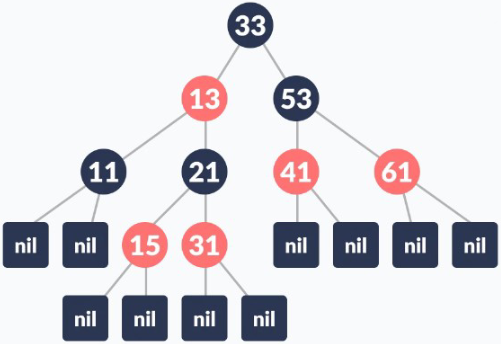
\includegraphics[width=0.7\textwidth]{image/RB-Tree.png} \\ \\
    \end{tabular}
\end{center}
Le operazioni degli RB-Tree saranno chiaramente simili a prima, in particolare:
\begin{itemize}
    \item \verb|Search|
    \item \verb|Max|
    \item \verb|Min|
    \item \verb|Successor|
    \item \verb|Precessor| (se $x$ ha 2 figli, il suo predecessore è il valore max nel suo sottoalbero sx e il suo successore il valore min nel suo sottoalbero dx. Se non ha un figlio a sx, il predecessore di un nodo è il suo primo antenato a sx)
    \item \verb|Insert| (difficile mantenere la colorazione)
    \item \verb|Delete| (difficile mantenere la colorazione)
\end{itemize}
La complessità delle operazioni è sempre data dall'altezza $h$ dell'albero, come $h = O(\log(n))$ con $h \leq 2 \log_2 (n+1)$. \\~\\

\subsection{Rotation}
Nell'operazione di \verb|Rotation|, le posizioni dei nodi di un sottoalbero vengono scambiate. \\
Esistono 2 tipi di rotazioni:
\begin{itemize}
    \item Rotazione a sx: la disposizione dei nodi a dx viene trasformata in quella dei nodi a sx
\begin{mdframed}
\begin{lstlisting}[language=C]
Left(T,x)
1   y = x.right
2   x.right = y.left
3   x.right.p = x
4   Transplant(T,x,y)
5   y.left = x
6   x.p = y
\end{lstlisting}
\end{mdframed}
    \item Rotazione a dx: la disposizione dei nodi a sx viene trasformata in quella del nodo a dx
\begin{mdframed}
\begin{lstlisting}[language=C]
Right(T,y)
1   x = y.left
2   y.left = x.right
3   if x.right != T.NULL
4       x.right.p = y
5   x.p = y.p
6   if y.p == T.NULL
7       T.root = x
8   else if y == y.p.right
9       y.p.right = x
10  else y.p.left = x
11      x.right = y
12      y.p = x
\end{lstlisting}
\end{mdframed}
\end{itemize}
